%% Простая презентация с примером включения программного кода и
%% пошаговых спецэффектов
\documentclass{beamer}
\usepackage{fontspec}
\usepackage{xunicode}
\usepackage{xltxtra}
\usepackage{xecyr}
\usepackage{hyperref}
\setmainfont[Mapping=tex-text]{DejaVu Serif}
\setsansfont[Mapping=tex-text]{DejaVu Sans}
\setmonofont[Mapping=tex-text]{DejaVu Sans Mono}
\usepackage{polyglossia}
\setdefaultlanguage{russian}
\usepackage{graphicx}
\usepackage{listings}
\lstdefinestyle{mycode}{
  belowcaptionskip=1\baselineskip,
  breaklines=true,
  xleftmargin=\parindent,
  showstringspaces=false,
  basicstyle=\footnotesize\ttfamily,
  keywordstyle=\bfseries,
  commentstyle=\itshape\color{gray!40!black},
  stringstyle=\color{red},
  numbers=left,
  numbersep=5pt,
  numberstyle=\tiny\color{gray},
}
\lstset{escapechar=@,style=mycode}

\begin{document}
\title{Реализация алгоритма Ray Marching}
\author{Гурьев Василий Александрович\\{\footnotesize\textcolor{gray}{группа 241\\руководитель ст. преподаватель Литвинов Ю.В.
}}}
\institute{Санкт-Петербургский государственный университет}
\frame{\titlepage}

\begin{frame}\frametitle{Введение}
\begin{itemize}
    \item Задача - построение реалистичного 3D изображения.
    \item Решения -
    \begin{itemize}
        \item Ray Tracing
        \item Render 3D models
        \item ***
        \item Ray Marching
    \end{itemize}
\end{itemize}
\end{frame}

\begin{frame}\frametitle{Постановка задачи}
\begin{itemize}
    \item Исследовать алгоритм Ray Marching
    \item Реализовать данный алгоритм, а так же реализовать библиотеку с полезными функциями
    \item Реализовать небольшую IDE для сцен Ray Marching
    \item Оптимизировать выполнение сцен в IDE до выполнения в реальном времени.
\end{itemize}
\end{frame}

\begin{frame}\frametitle{Реализации алгоритма}
\begin{itemize}
    \item Коммерческие проекты
    \begin{itemize}
        \item Компьютерные игры
        \item Фильмы / мультфильмы
    \end{itemize}
    \item Аналогичные разработки
    \begin{itemize}
        \item Некоторые сайты для разработки шейдеров
        \item IDE для написания сцен при помощи RayMarching в открытом доступе я не нашел.
    \end{itemize}
\end{itemize}
\end{frame}

\begin{frame}[fragile]\frametitle{Ray Tracing}
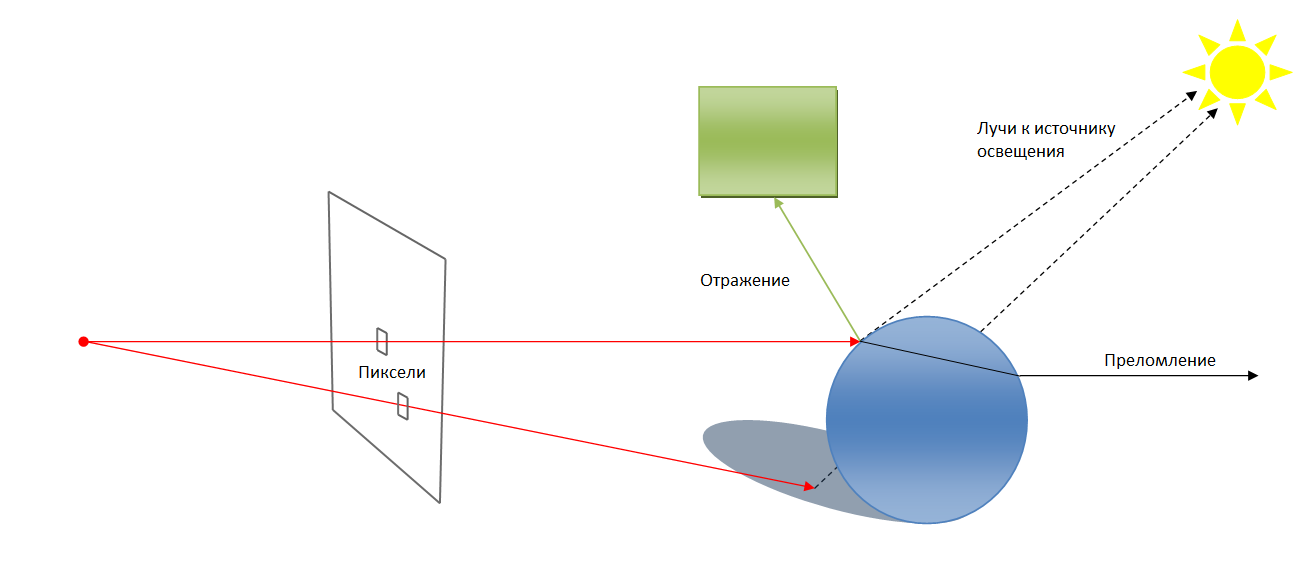
\includegraphics[width = 310pt]{raytrace.png}
\end{frame}

\begin{frame}[fragile]\frametitle{Ray Tracing}
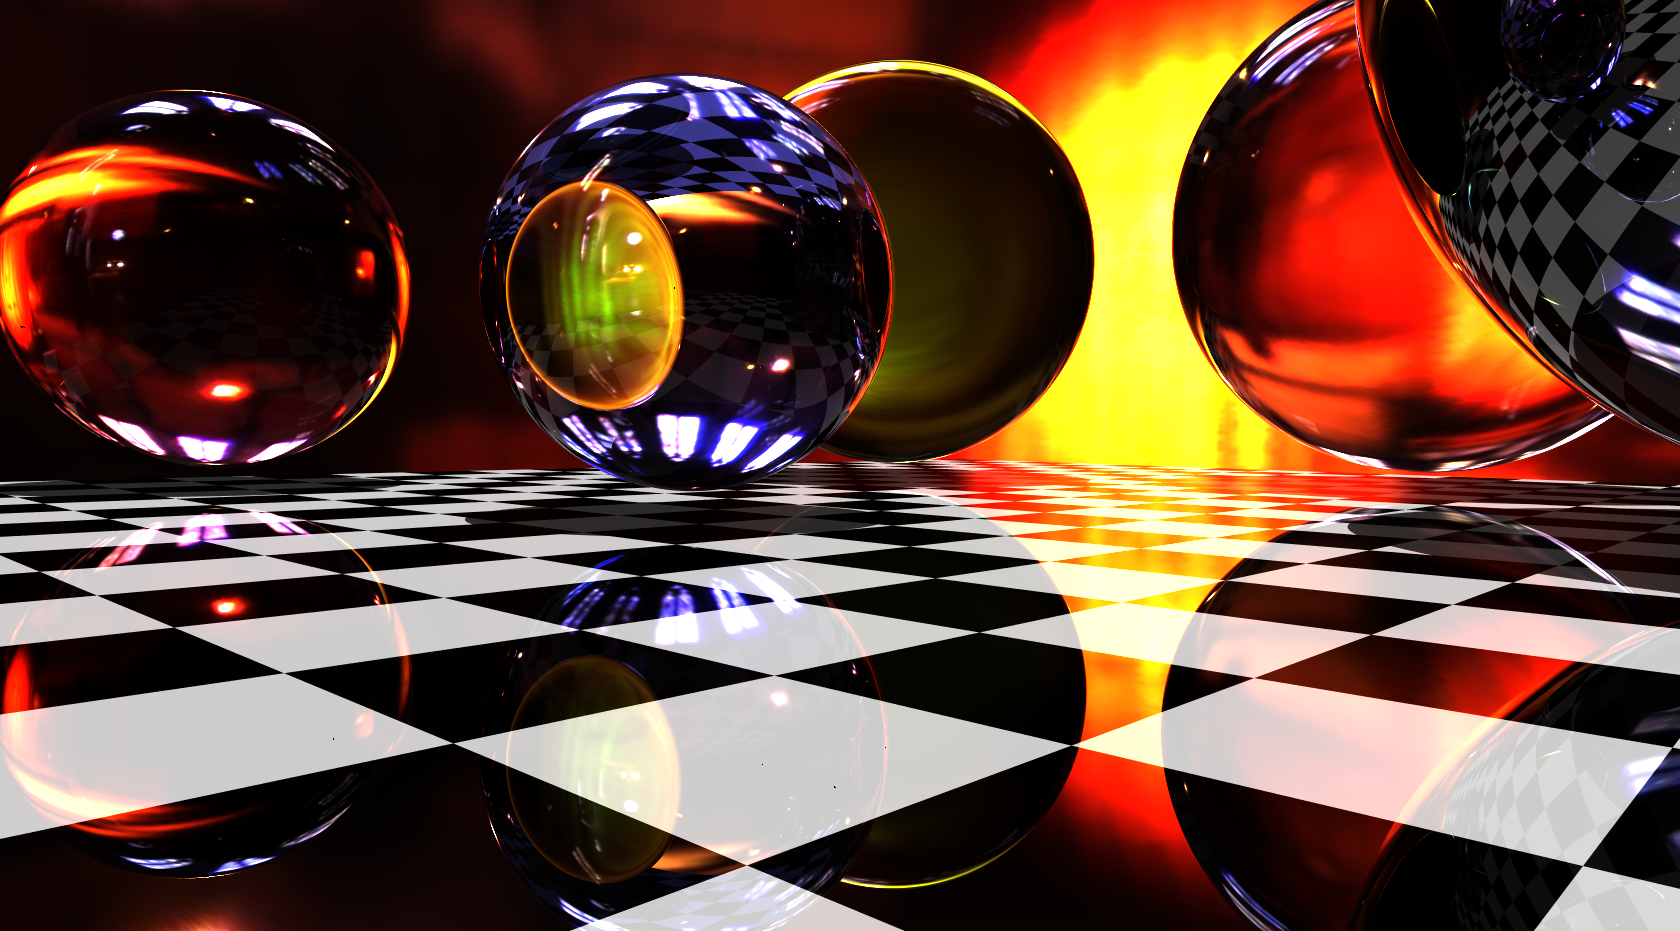
\includegraphics[width = 310pt]{scene.png}
\end{frame}

\begin{frame}\frametitle{Ray Marching}
\begin{itemize}
    \item Объекты задаются не аналитическим уравнением, а специальной функцией.
    \item Вместо аналитического поиска точки пересечения - трассировка по лучу.
\end{itemize}
\end{frame}

\begin{frame}[fragile]\frametitle{Ray Marching}
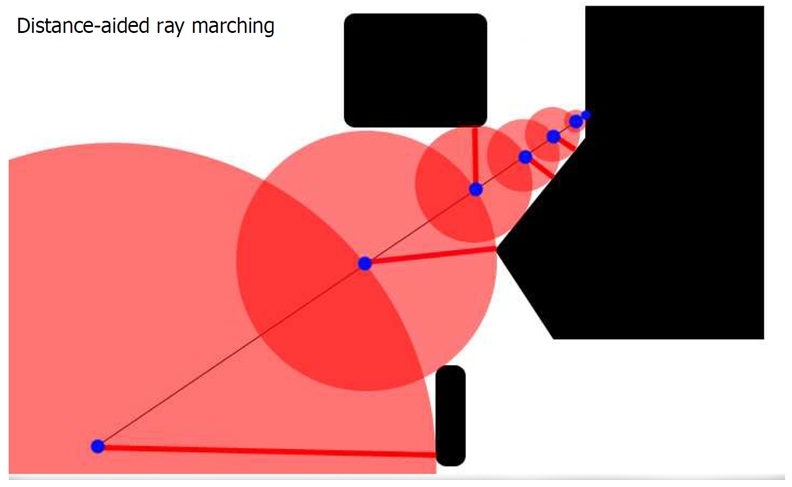
\includegraphics[width = 310pt]{ray.jpg}
\end{frame}

\lstset{language=c++}
\begin{frame}[fragile]\frametitle{Пример функции}
\begin{lstlisting}
float sdSphere(vec3 pos, float rad)
{
    return len(pos) - rad;
}

float sdTorus(vec3 pos, vec2 t)
{
    return len(vec2(len(pos.xz) - t.x, pos.y)) - t.y;
}

float sdUnionOfFigure(vec3 pos, vec2 t, float rad)
{
    return min(sdSphere(pos, rad), sdTorus(pos, t));
}
\end{lstlisting}
\end{frame}

\begin{frame}[fragile]\frametitle{Более сложный пример}
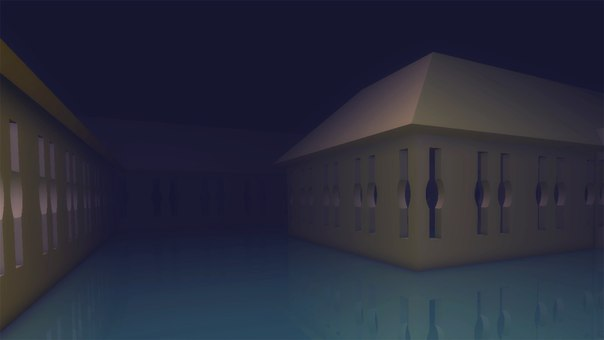
\includegraphics[width = 310pt]{house.jpg}
\end{frame}

\begin{frame}[fragile]\frametitle{Интересные эффекты}
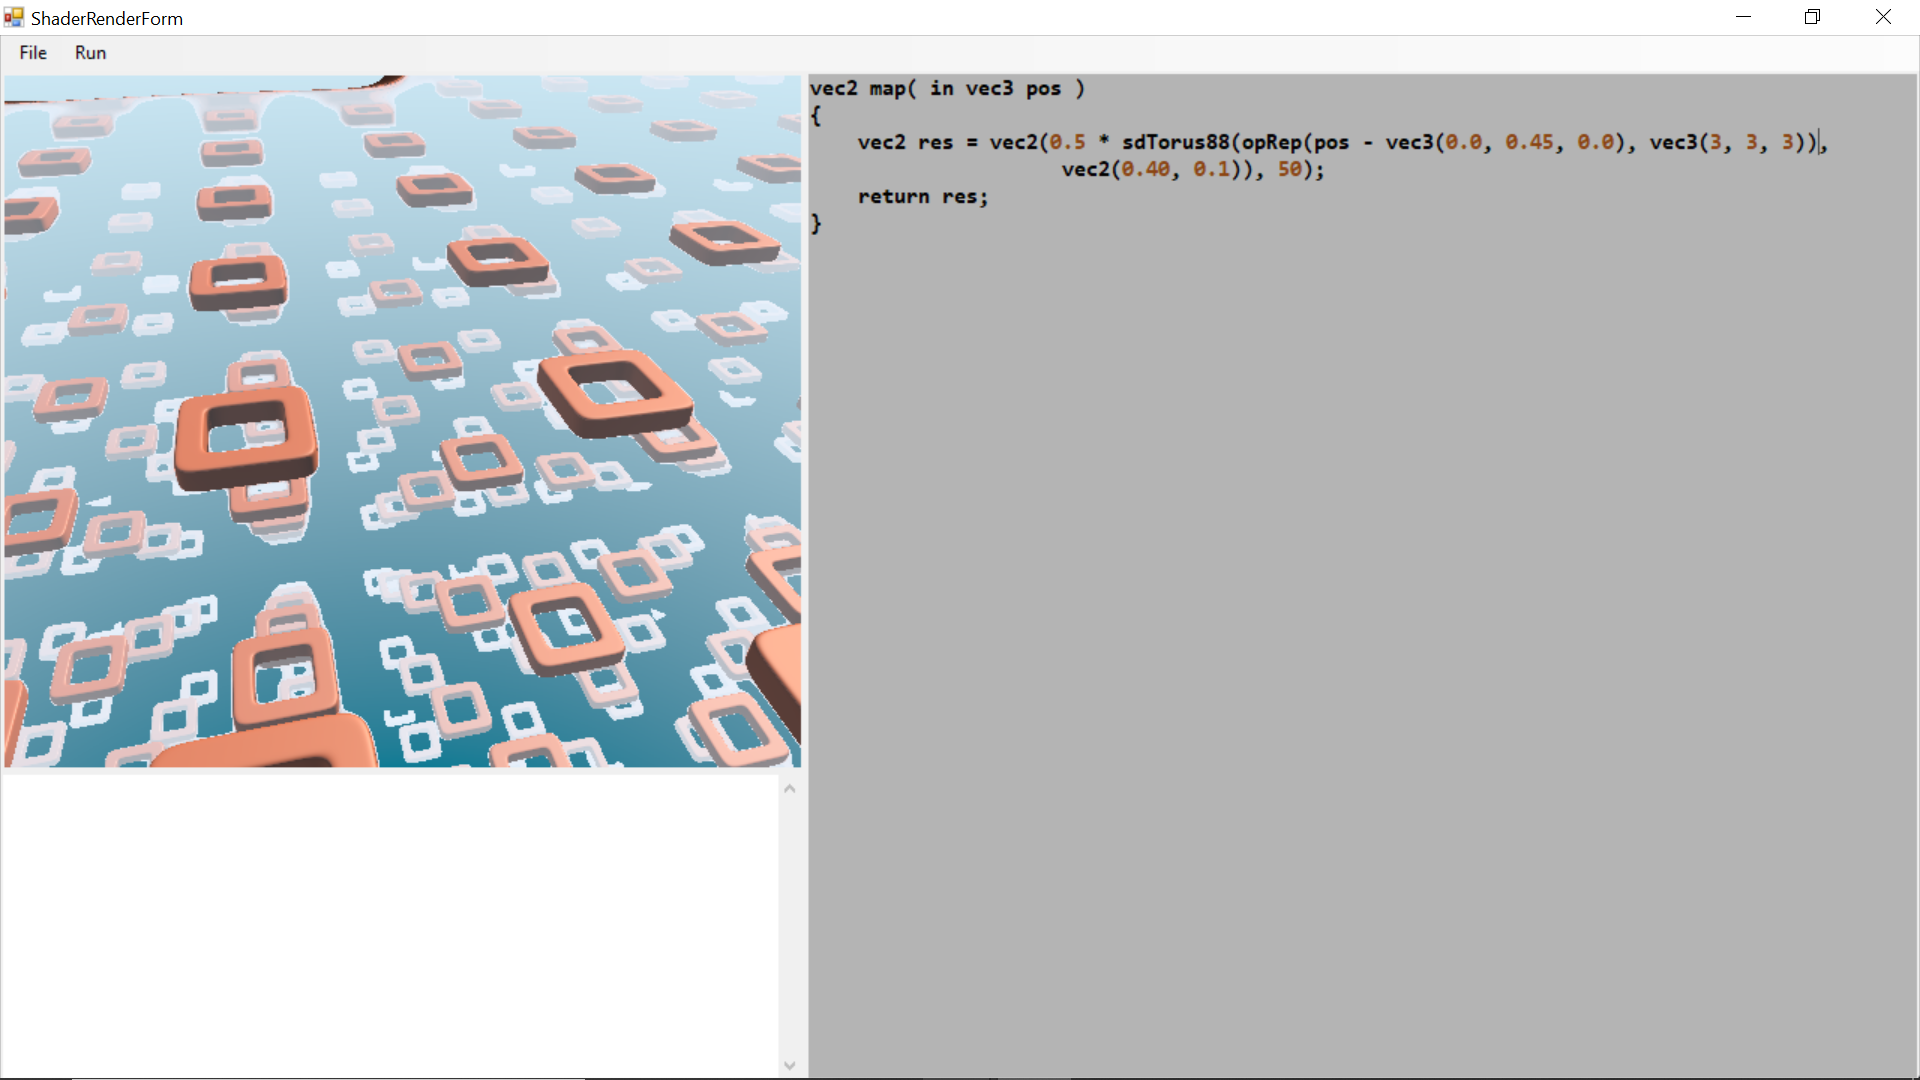
\includegraphics[width = 310pt]{replace.png}
\end{frame}

\begin{frame}[fragile]\frametitle{IDE}
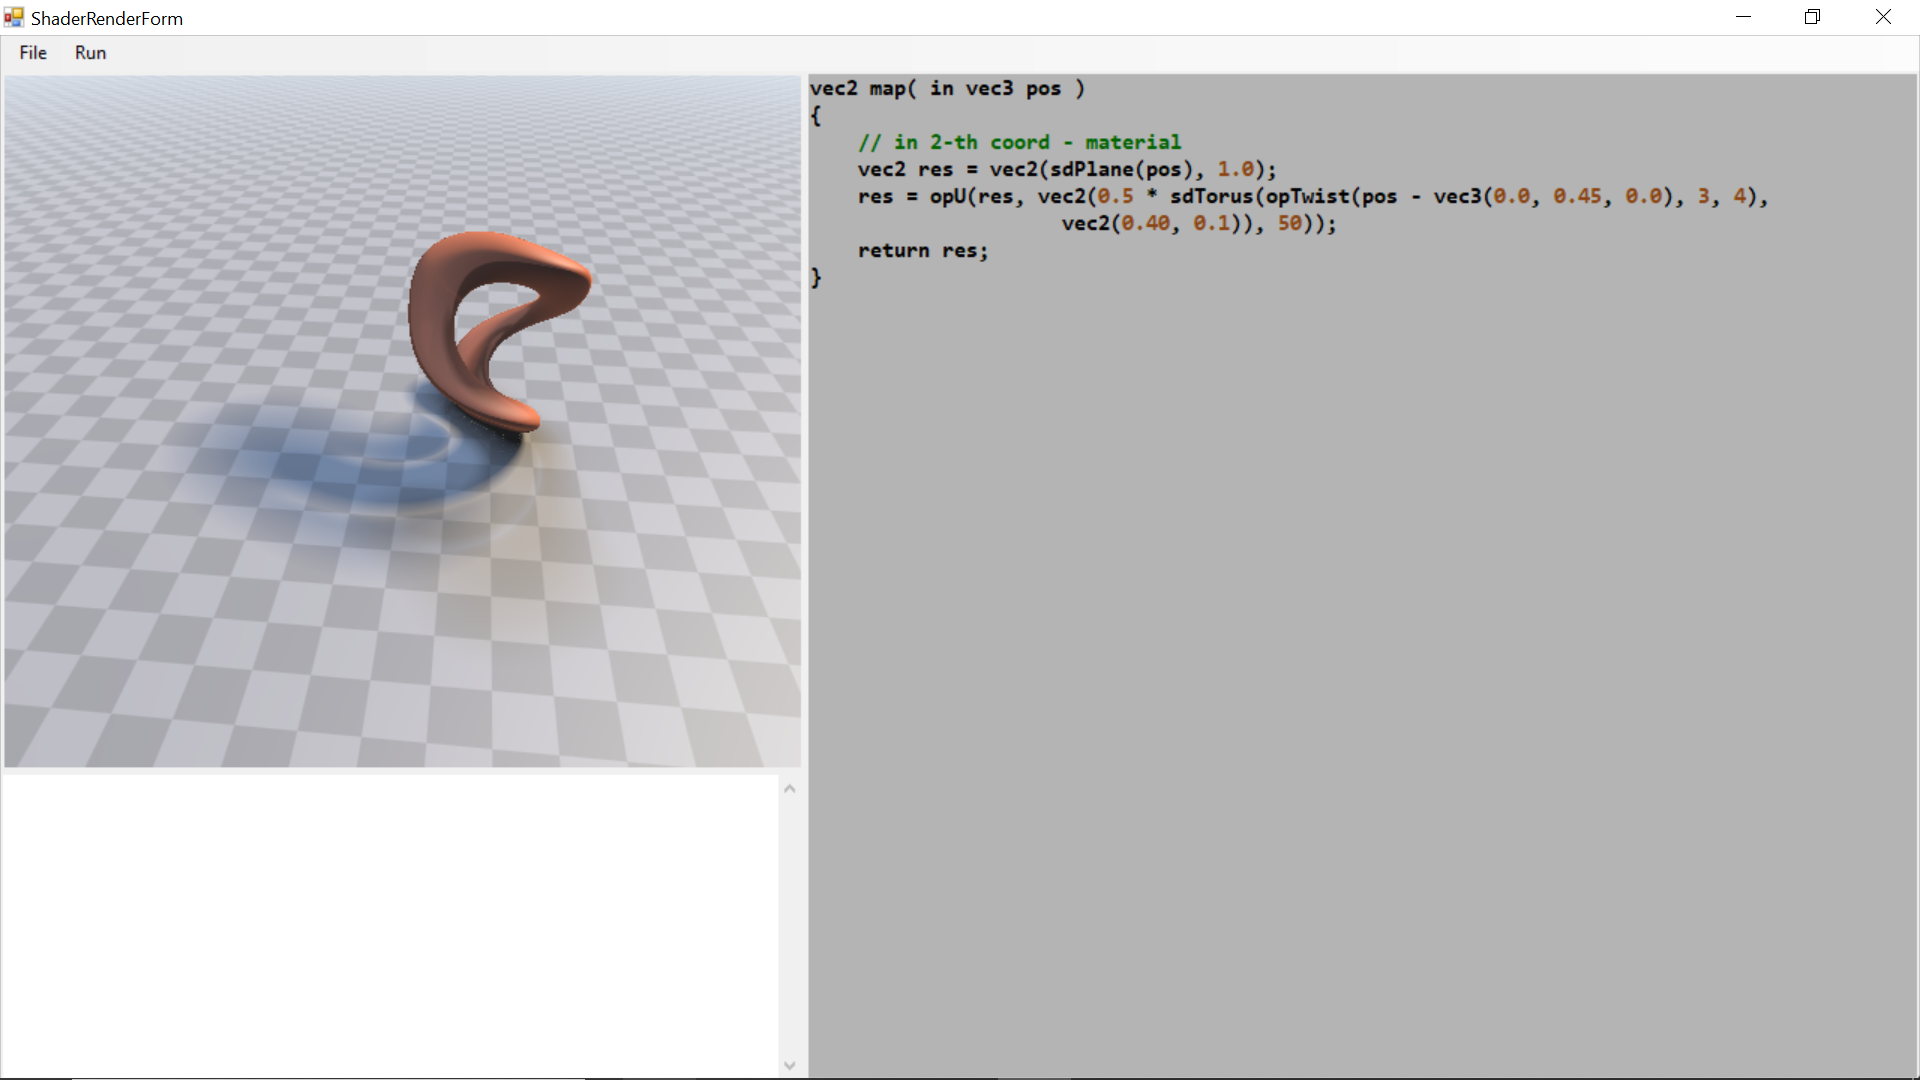
\includegraphics[width = 310pt]{prim1.png}
\end{frame}

\begin{frame}\frametitle{Оптимизация}
\begin{itemize}
    \item Получение цвета каждого пикселя картинки - независимая операция
    \item Обычное распараллеливание - неэффективно, распараллеливание на GPU работает гораздо быстрее
    \item Распараллеливание произвелось при помощи встроенных срадств OpenGL, а именно - пиксельных шейдеров
\end{itemize}
\end{frame}

\begin{frame}\frametitle{Результаты}
\begin{itemize}
    \item Исследован и реализован алгоритм Ray Marching
    \item Реализована библиотека с функциями для Ray Marching, так же поддержка освещения и мягких теней.
    \item Реализована небольшая IDE для сцен Ray Marching
    \item За счет выполнения на GPU сцены выполняются в реальном времени.
\end{itemize}
\end{frame}
\end{document}